\chapter{\label{ch2-mechanics} The Compact High Energy Camera}

\minitoc

\notes[inline,caption={}]{
	\section{Plan}
	\subsection{Topics}
	\begin{itemize}
		\item Introduce TARGET architecture \& Wilkinson ADC
		\item Different TARGET versions
		\item FEE
		\item MAPMs
		\item SiPMS
		\begin{itemize}
			\item How they work
			\item Comparison investigations
			\item Property trade-offs
		\end{itemize}
		\item CHEC-M
		\item Changes for CHEC-S
		\item Future - MUSIC ASICs
	\end{itemize}
	\subsection{Questions}
	\begin{itemize}
		\item ?
	\end{itemize}
}

\change[inline,caption={}]{
	\begin{itemize}
		\item number of pixels
        \item number of modules
        \item number of pixels per module
        \item number of cells
        \item pixel gaps
        \item module gaps
	\end{itemize}
}

\section{Introduction}

Due to the design of \gls{gct} as a dual-mirror Schwarzschild-Couder telescope, it is capable of a \SI{9}{\degree} \gls{fov} \change{intro: talk about benefit of high FoV} while simultaneously reducing the plate scale by a factor of $\sim 3$ compared to single-telescope designs. This large reduction in plate scale allows for a much more compact camera, for which novel opportunities in photosensor technology exist \cite{Vassiliev2007}. The camera that has been developed for \gls{gct} is appropriately known as the \glsf{chec}.

Two designs have been implemented for \gls{chec}, each featuring a different multi-pixel photon-counting sensor technology. A \glsf{mapmt} based camera known as \gls{chec-m} was the first to be commissioned, and received its inauguration on the \gls{gct} telescope structure at the Observatoire de Paris-Meudon in November 2015 \cite{Watson2017}. A second camera, known as \gls{chec-s}, is currently undergoing commissioning at the Max-Planck-Institut für Kernphysik in Heidelberg, Germany. This camera utilises \glsfpl{sipmt} as a photosensor. \gls{chec-s} also features upgrades the digitisation chain that were developed since the commissioning of \gls{chec-m}.

This chapter will describe the components of the \glsf{chec}, covering the photosensor, \gls{fee} and \gls{bee}. These descriptions will be focussed on the factors contributed by the electronics that have a significant influence on the low-level calibration and performance investigations covered in this thesis. Furthermore, the external components and laboratory set-up will be described. Finally, the data output of the camera is described, with specific focus on the characteristics of the waveform readout. The calibration and analysis of these waveforms obtained from the full camera electronics chain is the primary focus of this thesis.

\section{Photosensors}

For a photosensor to be useful to \glspl{iact}, it must be:
\begin{enumerate}
\item Sensitive to Cherenkov (blue) light.
\item Fast in its response to a signal, which is required to detect the prompt Cherenkov shower flashes.
\item Cheap, allowing large arrays of them to be combined to fill the full plate scale of the telescope and provide high spatial resolution of the shower.
\end{enumerate}

\subsection{Photomultiplier Tubes}

\begin{figure}
	\centering
    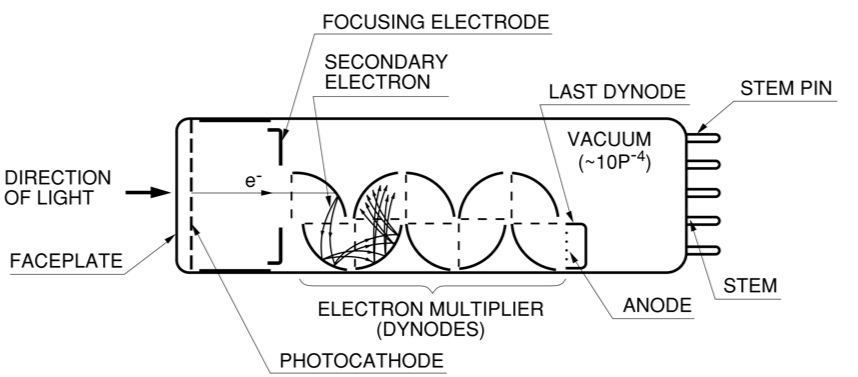
\includegraphics[width=\textwidth]{pmt} 
	\caption[Diagram of a Photomultiplier Tube.]{Common diagram of a Photomultiplier Tube (box-and-grid type) \cite{Hamamatsu2016}.}
	\label{fig:pmt}
\end{figure}

Since the inception of the Imaging Atmospheric Cherenkov Technique, the photosensors used for \gls{iact} cameras have almost exclusively been \glsfpl{pmt} \cite{Weekes2003}. These detectors operate as photon counting devices, where the charge produced by a single photon is amplified into a large current signal that can be read out. The components of a \gls{pmt} are as follows (using Figure~\ref{fig:pmt} for reference):
\begin{description}
\item [Photocathode] Produces electrons from incident photons via the photoelectric effect. These electrons are often referred to as ``photoelectrons''. Associated with a photocathode is its wavelength-dependant probability that photon will be converted into a photoelectron. This is known as its \gls{qe}, and is determined by the compound it is made of. The photocathodes in \glspl{pmt} are typically sensitive to visible light, with a \gls{qe} that peaks at \SI{\sim 30}{\percent} for \SI{\sim 400}{nm} (for the best photocathodes) \cite{Hamamatsu2016}.
\item [Focusing Electrode] Ensures that photoelectrons produced at the edges of the photocathode are focussed onto the first dynode.
\item [Electron Multiplier] The \gls{hv} across the \gls{pmt} accelerates the photoelectrons to the first dynode. Upon the impact, the dynode will release a further amount of electrons, the number of which is proportional to the kinetic energy of the incident electron. These secondary electrons are then accelerated to the next dynode, which has a higher voltage than the previous dynode. 
where $A$ 
\item [Anode] The total result of the dynode chain is a proportional amplification from the initial photocathode current $I_c$ to the output anode current $I_a$. The proportionality factor is known as the gain of the photomultiplier. The gain $G$ depends on the number of dynode stages $n$, and the value of high voltage applied $V$ \cite{Hamamatsu2016}:
\begin{equation} \label{eq:pmt_gain}
G = \frac{I_a}{I_c} = k V^{\alpha n},
\end{equation}
where $k$ is a constant that depends on the photomultiplier design, and $\alpha$ is a coefficient determined by the dynode material and geometric structure (typically has values around 0.7 to 0.8).
\end{description}

\begin{figure}
	\centering
    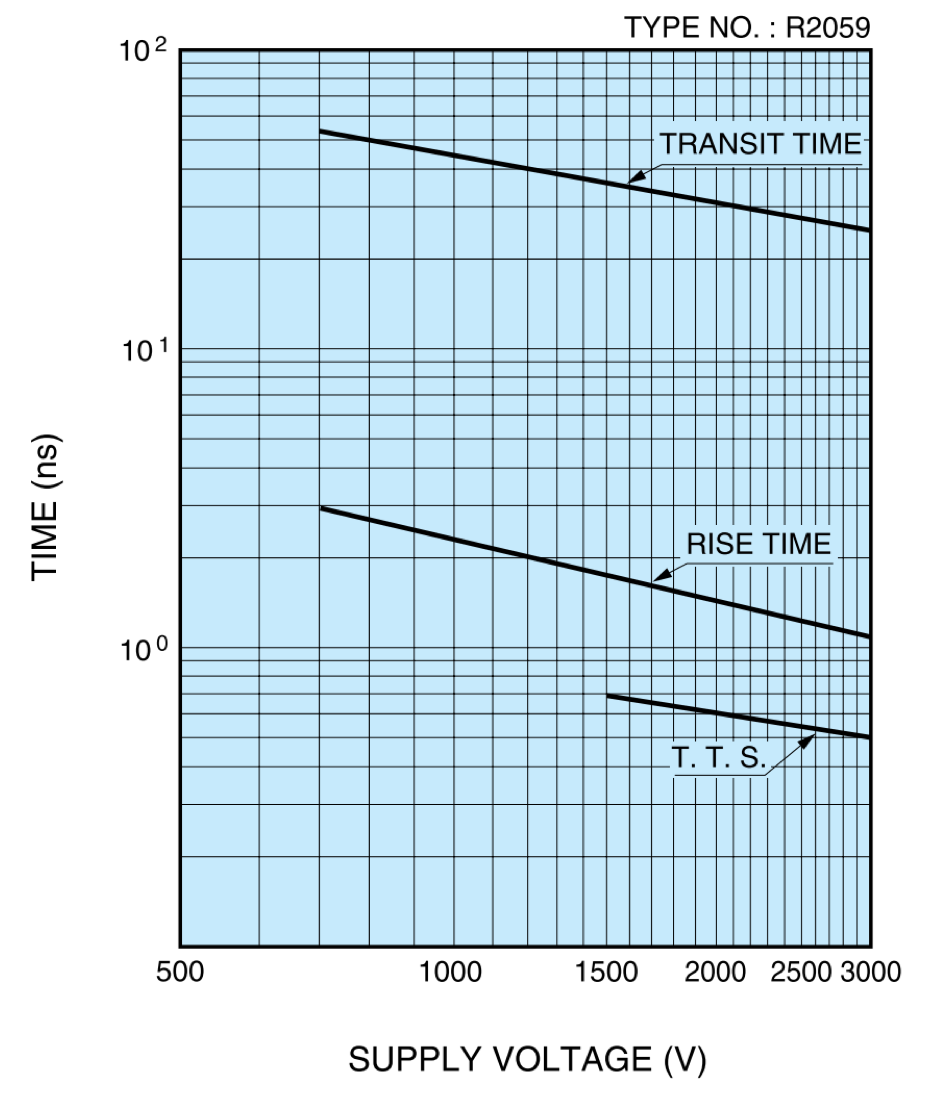
\includegraphics[width=\textwidth]{pmt_time} 
	\caption[Photomultiplier Tube timing characteristics.]{Typical values for the timing response of a Photomultiplier Tube \cite{Hamamatsu2016}.}
	\label{fig:pmt_time}
\end{figure}

Due to their wide usage across many fields, \glspl{pmt} are available at a very reasonable cost. The timing response of \glspl{pmt} faithfully reproduce the incident light pulse, however the anode's pulse rise time property does modify the response slightly \cite{Hamamatsu2016}. Additionally, there is a delay in signal due to the electron transit time along the dynode chain. This transit time has an associated ``transit time spread'' due to the different paths the electrons may take in the dynode chain. These time response characteristics are dependant on the dynode structure and applied voltage. Examples of the typical timing response values are shown in Figure~\ref{fig:pmt_time}.

Beyond their low \gls{qe}, a second disadvantage of a \gls{pmt} is its high voltage requirement \cite{Weekes2003}. Furthermore, since \glspl{pmt} generally have $\sim 10$ dynode stages, Equation~\ref{eq:pmt_gain} dictates that a small change in voltage will result in a large variation in gain. The high voltage supply therefore needs to be extremely stable \cite{Hamamatsu2016}. This is particularly unfavourable for the application of \glspl{pmt} in \glspl{iact}, due to the typical remoteness of the telescopes. A third disadvantage is the robustness of a \gls{pmt}, as they are very sensitive to light and can be permanently damaged if exposed to bright sources, such as the full moon. This disadvantage can limit the amount of observation time that is safe for the telescopes.

\subsection{Multi-Anode Photomultiplier Tubes}

\begin{figure}
	\centering
    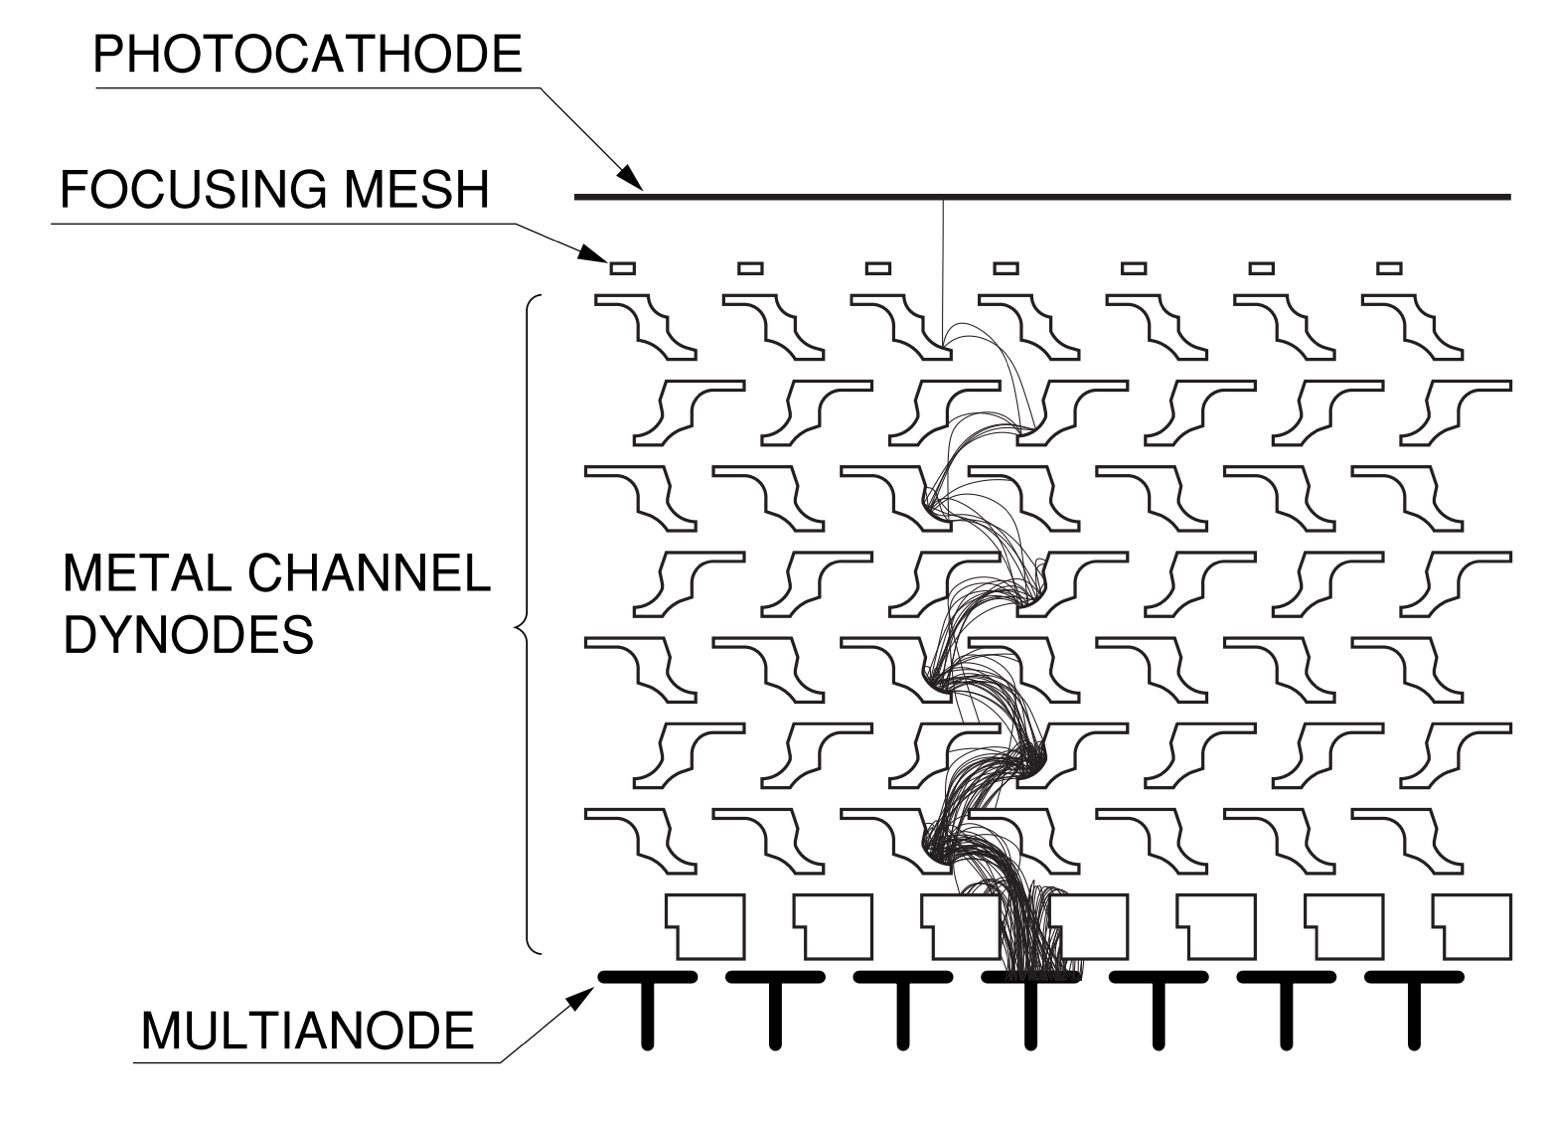
\includegraphics[width=\textwidth]{mapmt} 
	\caption[Internals of a Multi-anode Photomultiplier Tube.]{Electrode structure of a Multi-anode Photomultiplier Tube, demonstrating an example electron multiplication trajectory \cite{HAMAMATSU2007}.}
	\label{fig:mapmt}
\end{figure}

In order to be compatible with the reduced plate scale of the telescope, more compact options than \glspl{pmt} must be found. An extension to the \gls{pmt} technology is the \glsf{mapmt}. This photosensor consists of many \glspl{pmt} arranged in a compact grid to provide position-sensitive detection of light. A diagram of the internal dynode structure for \glspl{mapmt} is shown in Figure~\ref{fig:mapmt}. The chosen \gls{mapmt} model for \gls{chec-m} is the Hamamatsu H10966B . This flat panel type \gls{mapmt} features an 8~x~8 multianode, resulting in 64 pixels per \gls{mapmt}. The entire module's diameter is \SI{49}{mm}, while each pixel has a diameter of \SI{\sim 6}{mm}. It provides a \gls{qe} of \SI{\sim 30}{\percent} at \SI{400}{nm} wavelength, a typical gain of \SI{3.3 x 10^5}, and a typical anode rise time and transit time of \SI{0.4}{ns} and \SI{4}{ns}, respectively \cite{Hamamatsu2011}. 

\begin{figure}
	\centering
    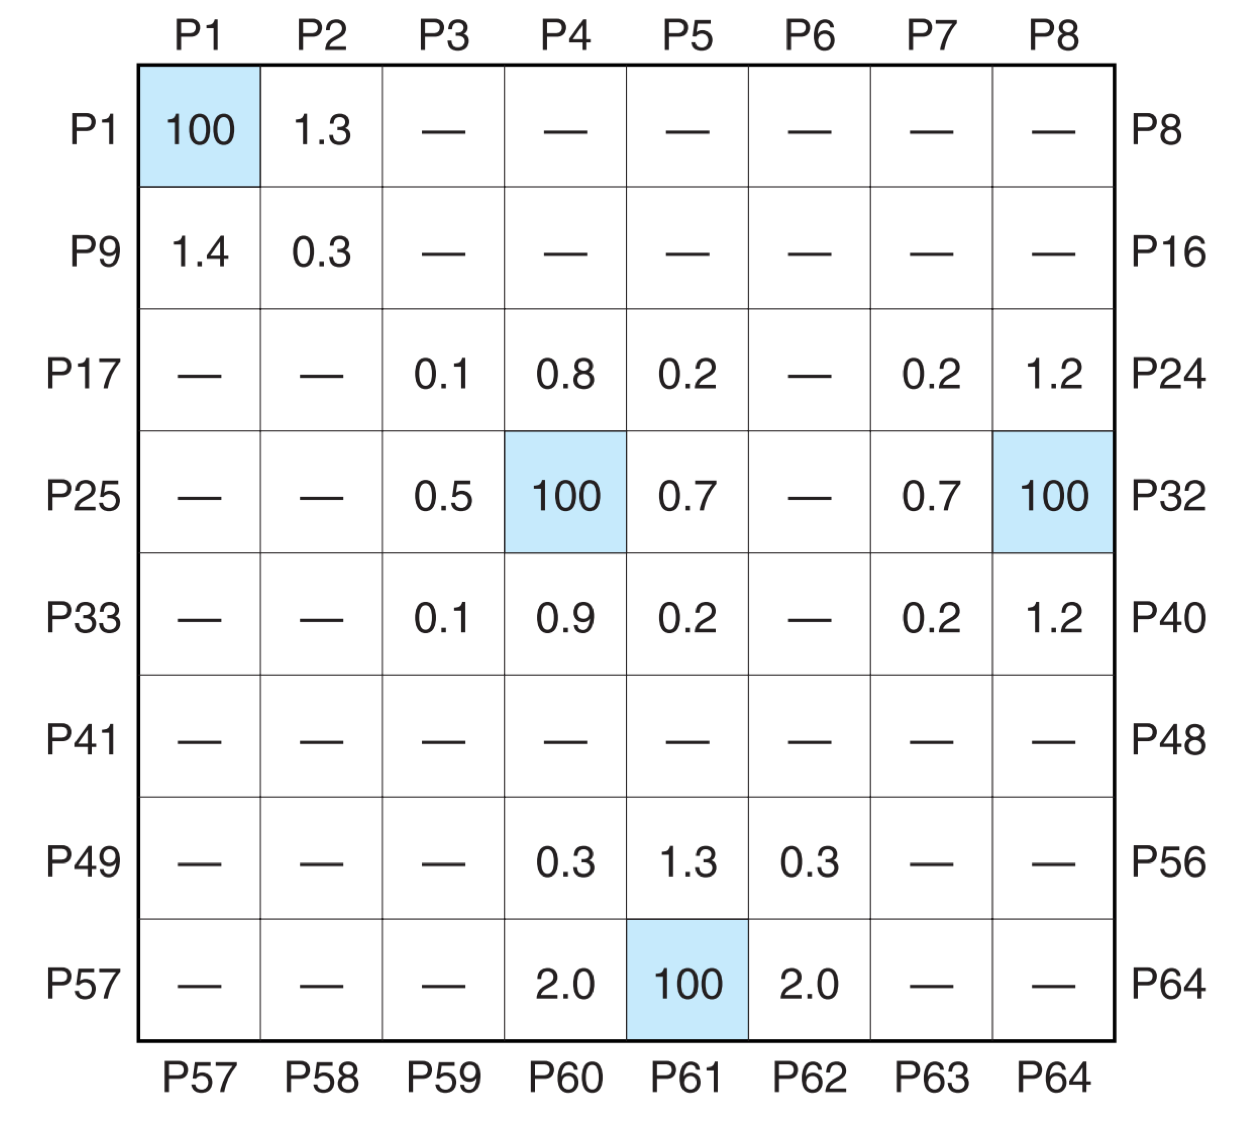
\includegraphics[width=\textwidth]{mapmt_crosstalk} 
	\caption[Multi-anode Photomultiplier Tube crosstalk.]{Example of the crosstalk present in an MAPMT, measured by using a fibre \cite{Hamamatsu2011}.}
	\label{fig:mapmt_crosstalk}
\end{figure}

An important concern when using an \gls{mapmt} is the crosstalk. This is the measure of how accurately the signal readout retains its positional information. It is hampered by the broadening of the electron flow in the photocathode and dynode chain. The crosstalk characteristics presented in the technical document for Hamamatsu H10966B are shown in Figure~\ref{fig:mapmt_crosstalk}.

\subsection{Silicon Photomultipliers}

For a photosensor to be considered as a replacement for the tried-and-trusted \gls{pmt} technology within \gls{iact} astronomy, it must deliver a higher \gls{qe} for a comparable cost. \glspl{sipmt}, or its solid state single photon detector precursors, have been actively developed since the 1960s \cite{Renker2006}. They have recently matured into a feasible replacement for traditional \gls{pmt} technology, causing a transitioning trend in the majority of fields that previously relied on \glspl{pmt}. 

\begin{figure}
	\centering
    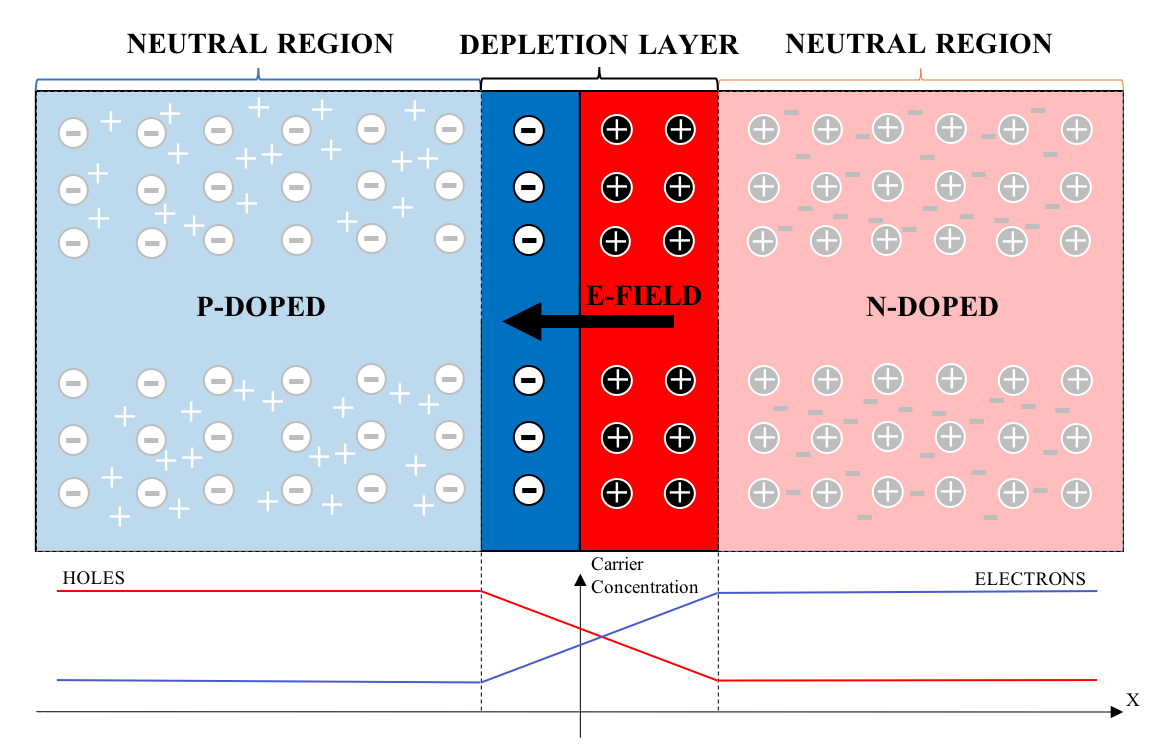
\includegraphics[width=\textwidth]{pn_junction} 
	\caption[A typical illustration of a P-N Junction.]{My own illustration of a P-N Junction, inspired by \textcite{Ghassemi2017}.}
	\label{fig:pn_junction}
\end{figure}

As with all solid state devices, the building blocks of \glspl{sipmt} are P-N Junctions. A p- and n-type material are created by the addition of impurities to a semiconducting material such as silicon. The impurities added to produce the n-type semiconductor increases its number of freely moving electrons, while the impurities added to produce the p-type semiconductor increases its number of freely moving holes. When the two materials are joined, the P-N Junction is formed. As a result of the abundance of charges in each material, a diffusion current forms with electrons moving from the n-type material (leaving behind its immobile positive ions) to combine with the holes in the p-type material. The same occurs vice versa for the excess holes in the p-type material, leaving behind its immobile negative ions. The result is a region adjacent to the junction with no free charges remaining, known as the depletion layer (Figure~\ref{}). 

These junctions are created through the contact

The major factors that now make \glsp{sipmt} an appealing replacement for \glspl{pmt}, as outlined by \textcite{Ghassemi2017}, are:
\begin{itemize}
\item The transition probability of a photoelectron from a silicon crystal’s valence band to its conduction band is higher than the emission probability achievable in an alkali-based photocathode. This factor results in a higher attainable \gls{qe}. 
\item The semiconductor properties of silicon enable a high collection efficiency of photoelectron charge, resulting in a reduced spread in the amplification of a single photoelectron in comparison to \glspl{pmt} (in the absence of optical crosstalk considerations, see Section~\ref{section:enf})
\item The high electrical conductance of doped silicon enables the low-voltage (of the order of \SIrange{10}{100}{V}) operation of an \gls{sipm}.
\item The high fill factor of \gls{sipmt} pixels and the compactness of the tiles allow a reduced dead space.
\item The mechanical reliability in terms of its ageing/warm-up considerations is much better than in \glspl{pmt}, as well as its performance in magnetic fields.
\end{itemize}





. while they have been utilised in high energy and medical fields for a while, they have only re

Form factor allows for a more compact module spacing 

% , a novel photosensor in the context of \gls{iact} astronomy, 



% despite their presence in the medical physics field for \change{find out value and reference}. \glspl{sipmt} operate on a \change{describe sipms, electron-hole} to detect photons. The appeal of \glspl{sipmt} are ..., therefore their adoption in many \gls{cta} cameras is anticipated. The \gls{chec-s} design is envisaged to be continued forward as the camera for \gls{gct}. Consequently, the commissioning and performance of \gls{chec-s} received the majority of focus within this thesis, however, a comparison to \gls{chec-m} is also provided at many stages.

\subsection{Excess Noise Factor} \label{section:enf}

\subsection{Future}

% \section{Pre-amplifiers and shapers}

% \section{Digitiser}

% \subsection{TARGET-5}

% \subsection{TARGET-C}

% \section{Back-End Electronics}

% \section{External Components}

% \subsection{LED Flashers}

% \subsection{Chiller}

% \section{Laboratory Set-Up}

% \section{Laboratory Calibration}

% \section{Readout Characteristics} \label{section:readout_characteristics}

% \change{define ADC}

% \change{monitoring information}

% \section{Nomenclature}

% \change[inline]{charge/signal, waveform/trace, events, noise (nsb/dcr/electronic/cosmic ray)}


% Traditionally, \glspl{iact} have relied on \glspl{pmt} as the photosensor. The fast, blue-sensitive, broadband light detectors provide photon


% In order to enable this compactness, while making no compromise to image resolution of the shower\change{need to understand pixel angular size, and the minimum needed to resolve the image} 

% ...tightly packed blue-sensitive photosensors with a physical diameter of \SI{\sim 6}{mm} diameter are relied upon. Additionally, in order to capture the short flash duration of the shower (typically only a few to a few tens of nanoseconds) the photosensors must be fast, and be coupled with high-speed digitising electronics. These two components, the photosensors and digitisers, are the defining characteristics of \gls{chec}.

% Two designs have been implemented for \gls{chec}, each utilising a different multi-pixel photon-counting sensor technology. A \glsf{mapmt} based camera known as \gls{chec-m} was the first to be commissioned, and received its inauguration on the \gls{gct} structure at the Observatoire de Paris-Meudon in November 2015 \cite{Watson2017}. A second camera referred to as \gls{chec-s} is currently undergoing commissioning at the Max-Planck-Institut für Kernphysik in Heidelberg, Germany. This camera utilises \glsfpl{sipmt}, a novel photosensor in the context of \gls{iact} astronomy, despite their presence in the medical physics field for \change{find out value and reference}. \glspl{sipmt} operate on a \change{describe sipms, electron-hole} to detect photons. The appeal of \glspl{sipmt} are ..., therefore their adoption in many \gls{cta} cameras is anticipated. The \gls{chec-s} design is envisaged to be continued forward as the camera for \gls{gct}. Consequently, the commissioning and performance of \gls{chec-s} received the majority of focus within this thesis, however, a comparison to \gls{chec-m} is also provided at many stages.




% %The re- quired compact nature of CHEC hinges on the use of com- mercially available multi-pixel photon-counting photosensors and the custom TARGET (TeV array readout with GSa/s sam- pling and event trigger) application-specific integrated circuits (ASICs) [21] to provide a high-performance low-cost solution

% \section{CHEC-M}

% \change[inline]{schematic illustration of electronics}

% \subsection{Multi-Anode Photomultiplier Tubes}

% \change[inline]{connection between gain and hv}
% \change[inline]{table of parameters}

% \subsection{Front-End Electronics}

% \subsubsection{Pre-Amplifiers}

% \subsubsection{TARGET}

% \begin{figure}
% 	\centering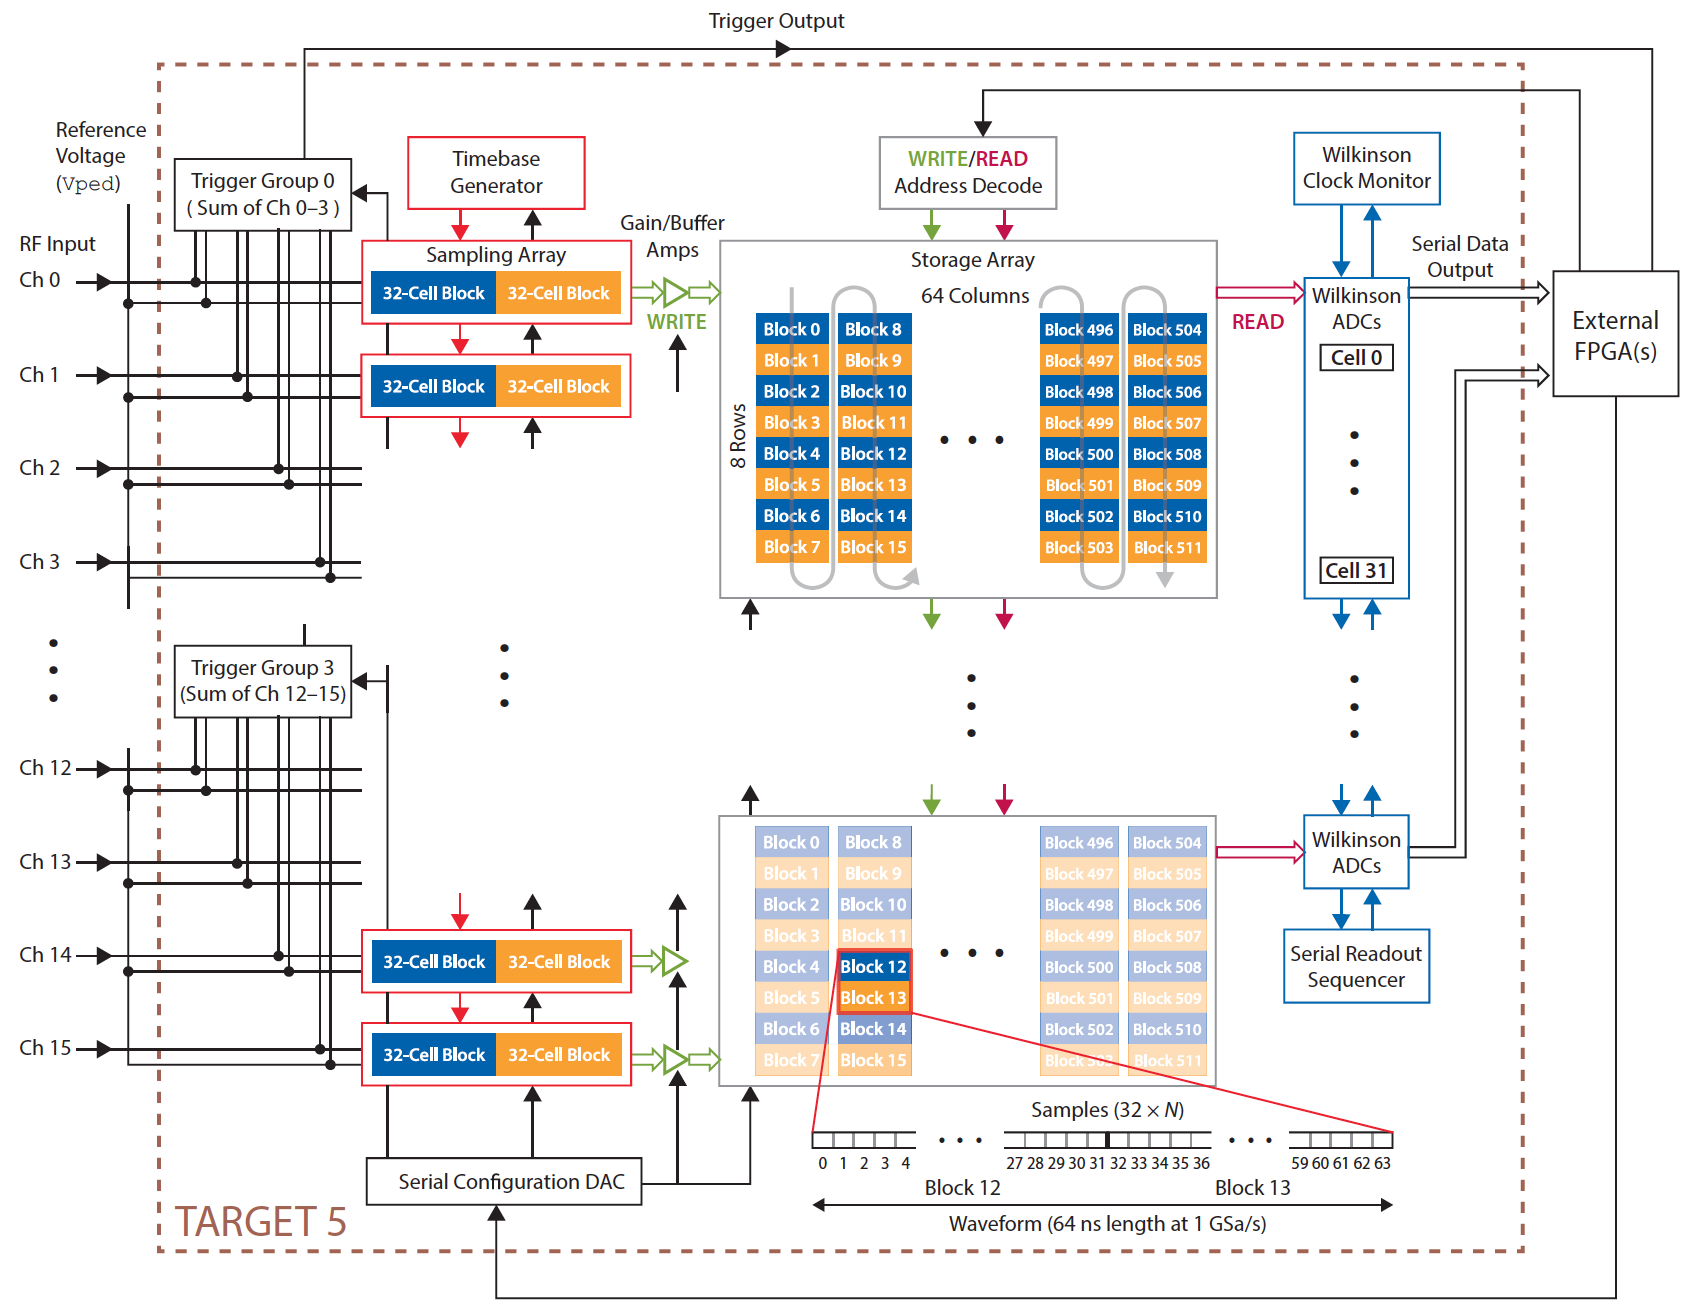
\includegraphics[width=\textwidth]{target5diagram} 
% 	\caption[Functional block diagram of the TARGET~5 ASIC.]{Functional block diagram of the TARGET~5 ASIC \cite{Albert2017} \change[inline]{Add more details}}
% 	\label{fig:target5diagram}
% \end{figure}

% \subsection{Back-End Electronics}

% \subsubsection{Backplane}

% \subsubsection{DACQ Boards}

% \section{CHEC-S}

% \notes{smaller gap between modules (and pixels?)}

% \subsection{Silicon Photomultipliers} \label{section:sipmts}

% \glspl{mapmt} have been the dominant photosensor within \gls{iact} astronomy since the beginning of the field \change{check book}. However, there has since been a huge amount of development in sensor technology to accommodate the advances in high energy particle and medical physics. \glspl{sipmt} are a novel technology to the \gls{iact} field. Originally designed for the use in \change{add uses}, they have previously been too \change{?} to be utilised for astronomy. Due to the latest improvements \change{talk about improvements} in \glspl{sipmt}, they are now being considered as an alternative to the long-standing \change{change word?} \glspl{mapmt} for \glspl{iact}. 

% The first \gls{iact} to 


% , with a potential to 

% \notes{see vinigrov for statement about enf, and how it could be worse for silicon even with the ``ultra- low excess noise of a limited Geiger mode avalanche multiplication'' due to opct. Make plot comparing the SPE response between sipm and mapm (essentially enf)}
% \notes{diagram of opct in silicon}
% \notes{four pixels combines - increases gain spread}

% \change[inline]{connection between gain and bias voltage}
% \change[inline]{table of parameters}
% \notes[inline]{Comparison in performance between CHEC-M and CHEC-S. show SPE spectrum again, huge decrease in spe\_sigma}

% % \change[inline,caption={}]{
% % 	\begin{itemize}
% % 		\item V_b bias voltage
% %         \item V_br breakdown voltage
% %         \item V_over Overvoltage
% %         \item PED does not change with temperature, but the breakdown voltage does, making it seem like the PDE changes
% % 	\end{itemize}
% % }

% \subsection{TARGET-C}

% \change[inline]{larger dynamic range, reference tf plot????}

% \change{name of TARGET-C FPGA?}

% \section{External Components} \label{section:external_components}

% \subsection{LED Flashers} \label{section:led_flashers}

% % Although not technically a part of the waveform processing chain, the LED flashers have an important role in the calibration system, especially for the final operation of the \gls{chec} cameras in \gls{cta}. Their purpose is to allow us to perform in situ calibration, by uniformly illuminating the camera via reflection in the secondary mirror. However, to achieve this, we must characterize and calibrate the LEDs such that we accurately know the illumination they are providing. \change[inline]{include some results on the LED calibration, and also mention their temperature dependence.}

% \subsection{Chiller}

% \section{Future} \label{section:checs_future}

% \subsection{Improvements in Silicon Photomultipliers}

% \notes[inline]{trenching, need to balance with PDE due to fill factor ?(VinigroV)}

% \subsection{MUSIC ASIC}

% \section{Laboratory Set-Up}

% \section{Laboratory Calibration} \label{section:lab-calib}

% In order to obtain reliable knowledge on the average illumination incident on the camera in our laboratory, it was necessary to calibrate the laser and filter wheel combination. This was of paramount importance for performing the camera flat-field calibration, and for obtaining a laboratory charge resolution result. There exists three stages required to achieve a calibration from filter-wheel position to average expected charge in each pixel:
% \begin{enumerate}
% \item Measuring the relationship between filter-wheel position and light transmissivity.
% \item Measuring the relative amount of light each pixel receives due to its position on the focal surface.
% \item Measuring an absolute illumination in photoelectrons for at least one filter-wheel position.
% \end{enumerate}
% Through combining the results of these stages, a conversion from filter-wheel position to expected number of photoelectrons in each pixel was obtained.

% \subsection{Filter Wheel}

% \begin{figure}
% 	\centering
%     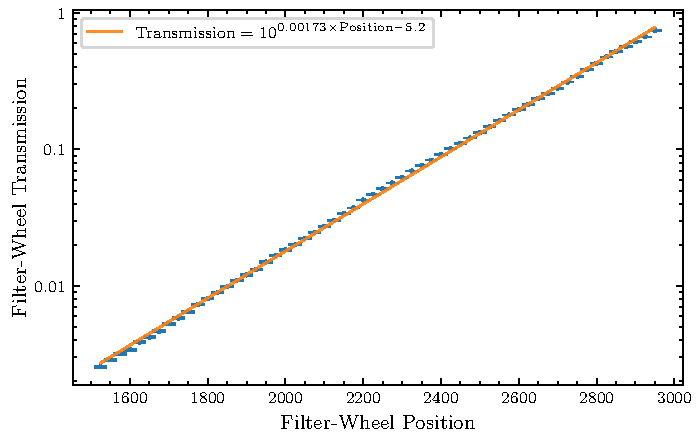
\includegraphics[width=\textwidth]{fw_position_justus} 
% 	\caption[Filter-wheel Position Calibration]{Logarithm of transmission versus position for the filter wheel. The relationship is fit with a straight line.}
% 	\label{fig:fw_position}
% \end{figure}

% \begin{figure}
% 	\centering
%     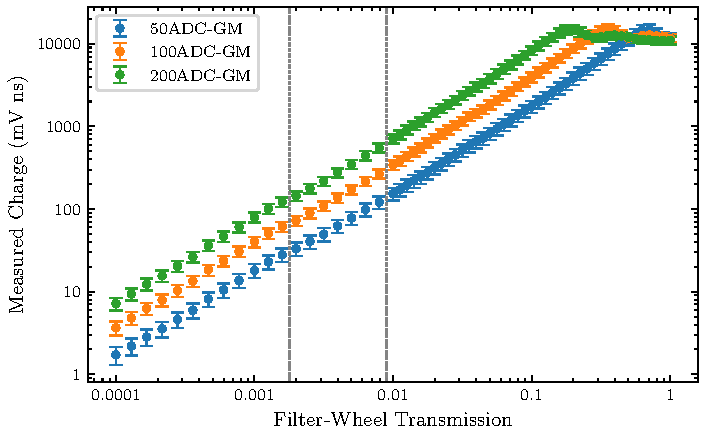
\includegraphics[width=\textwidth]{measured_versus_transmission} 
% 	\caption[Measured charge versus transmission]{Average charge across all CHEC-S pixels versus filter-wheel transmission. Three differently-gain-matched datasets are shown (50~ADC, 100~ADC, 200~ADC). Each gain matching results in a different bias voltage across the photosensor, and therefore a different gain, optical crosstalk, and PDE. Features shared between the datasets at a transmission value can only be due to errors in the filter-wheel calibration. Two clear features are highlighted by the vertical grey lines. Features shared at a measured charge value are due to shared properties in the Transfer Function (such as saturation).}
% 	\label{fig:measured_versus_transmission}
% \end{figure}

% \begin{figure}
% 	\centering
%     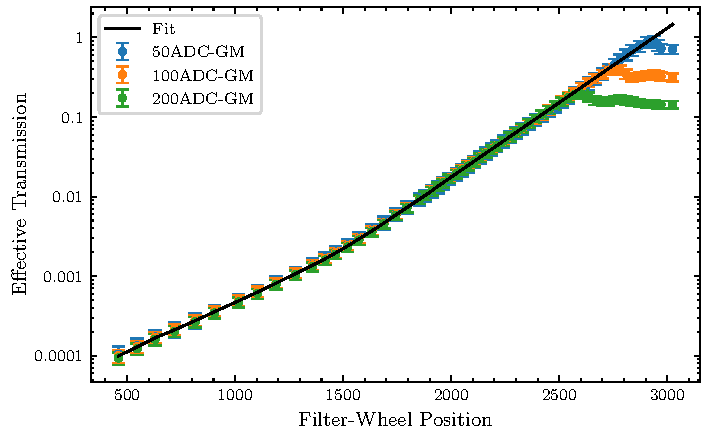
\includegraphics[width=\textwidth]{fw_correction} 
% 	\caption[Secondary filter-wheel calibration]{The measured charges from Figure~\ref{fig:measured_versus_transmission} converted into an ``effective transmission'', providing a filter-wheel calibration that is corrected for artefacts resulting from the first stage of calibration.}
% 	\label{fig:fw_correction}
% \end{figure}

% The calibration of the filter wheel was performed in two stages: an initial measurement with a reference \gls{sipmt} in order to obtain an approximate handle on the relative illumination, and a secondary correction using the camera at different gain settings.

% \subsubsection{Reference SiPMT}

% Using a single reference silicon photomultiplier pixel connected to an oscilloscope, centred on the camera focal plane, the ratio between the signal with and without the neutral-density filter was calculated for different filter-wheel positions (i.e. different attenuations). As the dynamic range of the reference \gls{sipmt} was limited, in order to cover the full range of filters attenuations, three approaches were utilised:
% \begin{enumerate}
% \item \textbf{Low-range} - Average illumination obtained from \gls{spe} spectrum, with a pre-amplifier attached to the \gls{sipmt}.
% \item \textbf{Mid-range} - Average pulse area, with a pre-amplifier attached to the \gls{sipmt}.
% \item \textbf{High-range} - Average pulse area, with no pre-amplifier attached.
% \end{enumerate}
% The overlapping values from each method were used to stitch the datasets together. The resulting points, shown in Figure~\ref{fig:fw_position}, were then used as a lookup table for the conversion from filter-wheel position to transmission.

% \subsubsection{Camera Correction}

% When looking at the average measured charge across the camera as a function of transmission, for three datasets where each has different bias voltages applied to the photosensors, features that share a position on the X axis can only occur from artefacts of the previous filter-wheel calibration. Figure~\ref{fig:measured_versus_transmission} indicates some of the artefacts which are easy to see. The measured charge was then converted into an ``effective transmission'' using the relation in Figure~\ref{fig:measured_versus_transmission}. By plotting the ``effective transmission'' against filter-wheel position, a new conversion from filter-wheel position to transmission was obtained from the fit shown in Figure~\ref{fig:fw_correction}.

% \subsection{Illumination Profile} \label{section:illumination_profile}

% Two contributions influence the relative amount of light each pixel receives, depending on its position on the camera focal surface. The first is due to the laser uniformity characteristics, the second is due to the curved focal surface of the camera.

% \subsubsection{Laser Profile}

% \begin{figure}
% 	\centering
%     %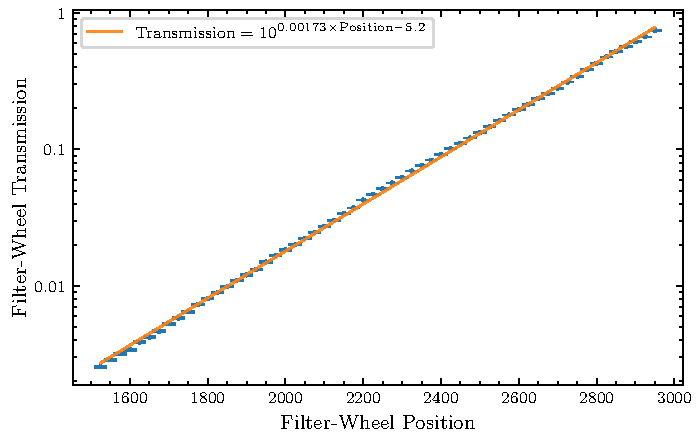
\includegraphics[width=\textwidth]{fw_position_justus} 
% 	\caption[Lab laser profile]{Spatial profile of the laser illumination along a flat plane in front of the camera, measured with a single reference \gls{sipmt} pixel attached to a robot arm. \change[inline]{Show value in each position, and then gradient fit?}.}
% 	\label{fig:light_profile}
% \end{figure}

% Despite attempts to homogenise the illumination from the laser-diffuser combination, there are still non-uniformities in the light received at the camera pixels that needed to be accounted for in the calibration. As shown in Figure~\ref{fig:light_profile}, a linear gradient in laser illumination exists across the x-y plane. This was found by attaching a single silicon photomultiplier pixel to a robot arm, and placing it at the camera position in from of the laser. Through the use of a single pixel, the amplitude measured is disentangled from the relative PDE. This pixel was then moved to each x-y position to calculate the ratio in signal amplitude, returning back to the origin to obtain a fresh value for comparison, thereby correcting for any deviations that may have occurred due to a change in temperature. The resulting distribution of ratios was fit with a linear gradient across the plane.

% \subsubsection{Camera Geometry}

% \begin{figure}
% 	\centering
%     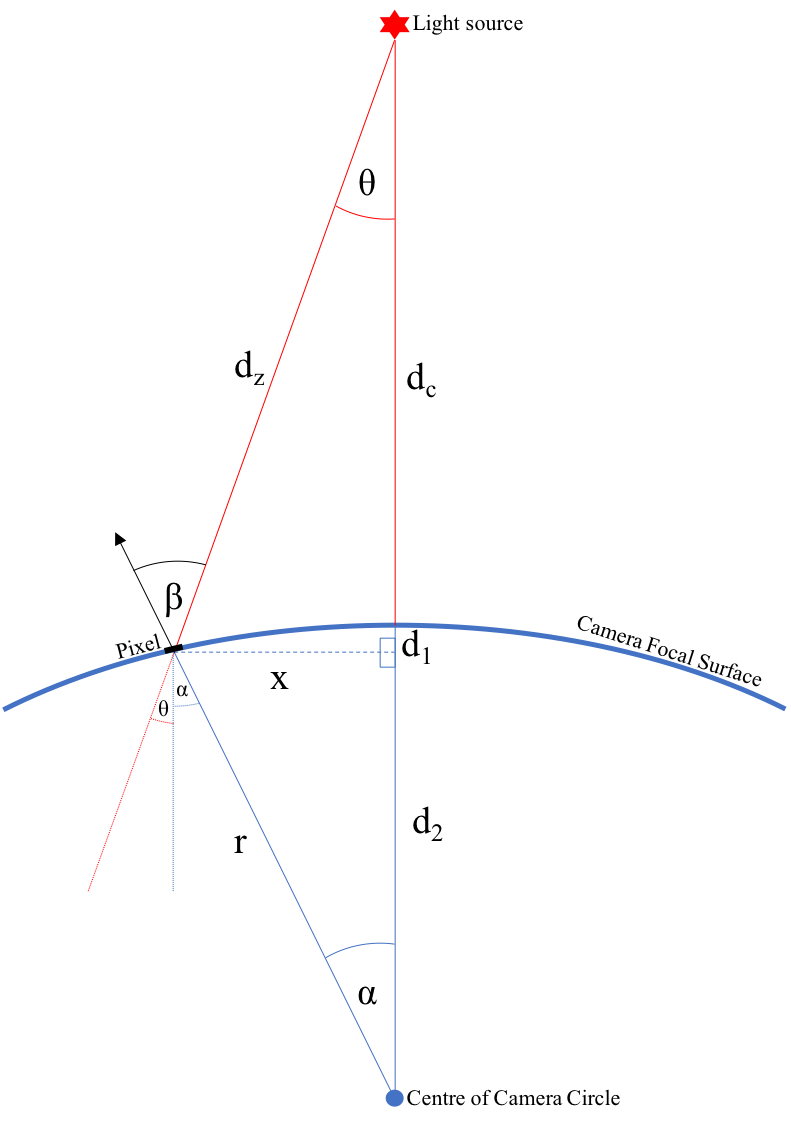
\includegraphics[width=0.75\textwidth]{laser_geometry} 
% 	\caption[Camera geometry correction schematic]{Two-dimensional geometry schematic of the laboratory set-up for uniform camera illumination, used to calculate the reduction in light level for each pixel depending on its distance from the camera centre.}
% 	\label{fig:laser_geometry}
% \end{figure}

% \change[inline]{Talk about how this is an approximation - modules are fixed along focal plane, light-source is somewhat between pointlike and at infinity, quote percentage that difference makes}

% \change[inline]{Add not to scale on figure}

% Due to the spherical camera focal surface, each pixel is at a different distance $d_z$ from the light-source, and therefore receives a different amount of light depending on its distance $x$ from the camera centre. Furthermore, at a ``viewing angle'' $\beta$, i.e. the angle between the normal to the pixel and the light-source, the amount of surface area of the pixel $A_P$ visible to the light-source is reduced. The visible surface area is known as the ``viewing area'' $A_V$. The combined geometric correction to the light intensity required to compensate for these effects is almost circularly symmetric, and therefore can be analytically approximated by using a two dimensional description of the camera, with a circular focal surface:

% \begin{equation} \label{eq:geom_distance1}
% d_1 = r - d_2 = r - \sqrt{r^2 - x^2},
% \end{equation}
% \begin{equation} \label{eq:geom_distance2}
% d_z = \sqrt{x^2 + (d_c + d_1)^2} = \sqrt{x^2 + (d_c + r - \sqrt{r^2 - x^2})^2}.
% \end{equation}
% \begin{equation} \label{eq:viewing_area1}
% \beta = \theta + \alpha = \sin^{-1}{\frac{x}{d_z}} + \sin^{-1}{\frac{x}{r}},
% \end{equation}
% \begin{equation} \label{eq:viewing_area2}
% \frac{A_V}{A_P} = \cos{\beta},
% \end{equation}
% \begin{equation} \label{eq:geom_correction}
% \frac{I_x}{I_c} = \frac{d_z^2}{d_c^2} \times \cos{\beta},
% \end{equation}
% where $A_P$ is the pixel area, $I_x$ is the intensity measured at the position of the pixel, $I_c$ is the intensity measured at the centre of the camera, and the remaining distances and angles are shown in Figure~\ref{fig:laser_geometry}.

% The resulting geometry corrections to the intensity for each pixel, arising from Equation\ref{eq:geom_correction}, can be seen in Figure~\change{add figure}. 

% The final illumination profile correction, combining both the laser profile and camera geometry, is shown in Figure~\change{add figure}. The description used for this calibration is only an approximation to the lab set-up. The following factors cause deviations from this model:
% \begin{itemize}
% \item The pixels are not precisely aligned on the spherical focal surface; the pixel angle is fixed to its module's angle. The modules are aligned on the spherical focal surface.
% \item The light source is not point-like. It produces a diffuse emission, which likely reflects along the walls of the box.
% \end{itemize}
% A future study could further improve on the models used for the illumination correction.

% \subsection{Absolute Illumination} \label{section:absolute_illumination}

% \begin{figure}
% 	\centering
%     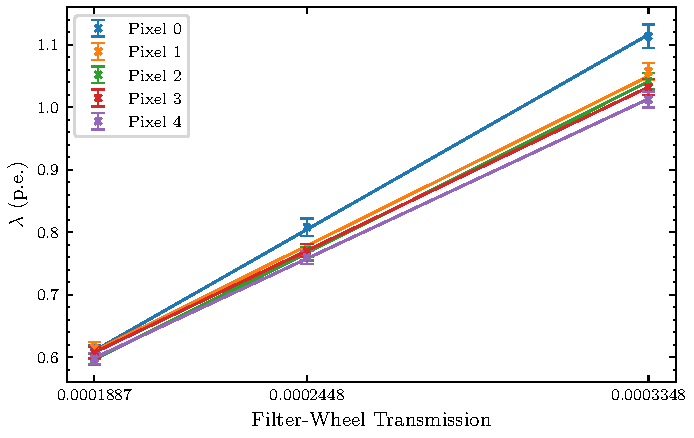
\includegraphics[width=\textwidth]{fw_calibration_fit} 
% 	\caption[Obtaining relationship between filter-wheel transmission and average illumination.]{Example of the linear regression to obtain the relationship between filter-wheel transmission and average illumination in photoelectrons ($\lambda$), for 5 pixels. The values of $\lambda$ are obtained from the simultaneous fits to the \gls{spe} spectra (Appendix~\ref{a1-spe}). The error bars on the points are the \si{1}{$\sigma$} parabolic errors obtained from the covariance matrix of the fit)}
% 	\label{fig:fw_calibration_fit}
% \end{figure}

% The method adopted to obtain a value for the absolute illumination was to use a fit to the \gls{spe} spectrum resulting from low-amplitude illumination of the pixels. Contained within this fit is the average illumination parameter, $\lambda$. The concept of the \gls{spe} fit is further covered in Chapter~\ref{ch5-calibration} and Appendix~\ref{a1-spe}.

% By simultaneously fitting three illuminations, we obtained three values of $\lambda$ per pixel. With the three filter-wheel transmissions (corresponding to the three illuminations) on the x-axis, these values of $\lambda$ were linearly regressed (weighted by the \si{1}{$\sigma$} parabolic error of the fit, $\sigma_\lambda$) to obtain the gradient $M_\lambda$ and y-intercept $C_\lambda$ per pixel. This linear regression is shown in Figure~\ref{fig:fw_calibration_fit}. The y-intercept represents the value of $\lambda$ one would get with zero filter-wheel transmission, and therefore indicates the \gls{nsb} and \gls{dcr}. The variation in $M_\lambda$ across the pixels arises from the folding of the illumination profile and the relative \gls{pde}. Therefore, the next step was to correct for the illumination profile contribution to the gradient. The resulting spread of $M_\lambda$ is solely from the relative \gls{pde} (Figure~\change{add figure, in this chapter or results chapter?}). The calibration from filter-wheel transmission $T_\text{FW}$ to the average illumination across the whole camera $\average{I}_{pe}$ is then obtained by taking the averages of the linear regression coefficients:

% \begin{equation} \label{eq:average_camera_illumination}
% \average{I}_{pe} = \average{M}_\lambda T_\text{FW} + \average{C}_\lambda,
% \end{equation}

% \subsection{Average Expected Charge}

% \begin{figure}
% 	\centering
%     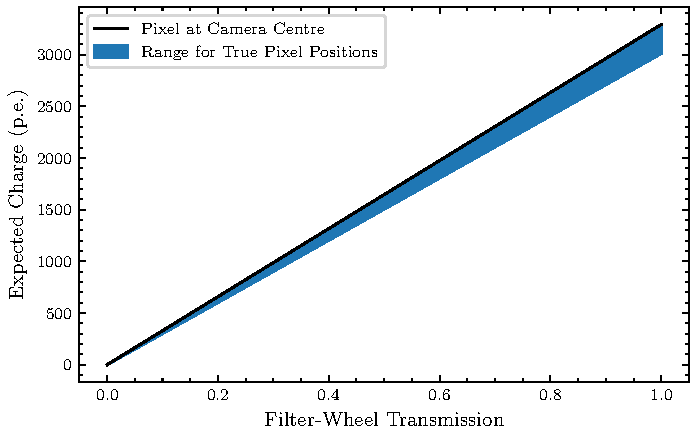
\includegraphics[width=\textwidth]{fw_calibration} 
% 	\caption[Calibration from filter-wheel transmission to expected charge]{Relationship between filter-wheel transmission and average expected charge in photoelectrons resulting from the filter-wheel calibration. The black line shows the conversion for a theoretical pixel positioned exactly at the camera centre. The error bars are calculated from the weighted standard deviation of the gradient estimates between the pixels, explained in Section~\ref{section:fwerr}}
% 	\label{fig:fw_calibration}
% \end{figure}

% As we corrected for the \gls{nsb} in the extracted signal value (Section~\ref{section:photosensor_calib}), the \gls{nsb} contribution to Equation~\ref{eq:average_camera_illumination} ($\average{C}_\lambda$) is subtracted to give us the charge we expect when illuminating the camera with a filter-wheel transmission $T_\text{FW}$, for a theoretical pixel perfectly positioned at the camera centre. This relation is shown in Figure~\ref{fig:fw_calibration}. To obtain the average expected charge $Q_\text{Exp}$ for each true camera pixel, this relation must be folded with the illumination profile correction factor $F_\text{pix}$:
% \begin{equation} \label{eq:average_expected_charge}
% Q_\text{Exp} = \average{M}_\lambda T_\text{FW}F_\text{pix}.
% \end{equation}
% This expression is important for the flat-fielding calibration (Chapter~\ref{ch5-calibration}) and the calculation of the \textit{Charge Resolution} for lab measurements (Chapter~\ref{ch7-performance}), as it tells us for a certain pixel and filter-wheel transmission, what charge we should expect to measure on average.

% \subsection{Consideration of Errors and Uncertainty} \label{section:fwerr}

% When performing the weighted linear regression between $\lambda_i$ and filter-wheel transmission $T_{FW_i}$ (with weights $w_i = \frac{1}{\sigma_{\lambda_i}^2}$ accounting for the parabolic error in $\lambda_i$), the standard error on the estimate of the gradient per pixel, $\sigma_{M_\lambda}$, can be calculated with the relation derived by \textcite{Taylor1997}:
% \begin{equation} \label{eq:wmerr}
% \sigma_{M_\lambda} = \sqrt{\frac{\sum w_i}{\sum w_i \sum w_i T_{FW_i}^2 - (\sum w_i T_{FW_i})^2}}, \quad i = 0, 1, 2, ..., N.
% \end{equation}

% During the correction for the illumination profile on the gradient estimates, the illumination correction factors were also applied to the standard error on the gradient estimate.

% While calculating the average gradient across the camera, $\average{M}_\lambda$, the individual gradient estimates were weighted by their corresponding standard error. To calculate an uncertainty on the resulting value for $\average{M}_\lambda$, the weighted standard deviation between the gradient estimates were also calculated. This uncertainty is illustrated in the error bars in Figure~\ref{fig:fw_calibration}. The resulting conversion value from filter wheel transmission to expected charge for a theoretical pixel located at the centre of the camera was calculated to be $\average{M}_\lambda = \SI[separate-uncertainty = true]{3253.76 \pm 305.32}{\pe}$\final{check value}.


% \section{Readout Characteristics} \label{section:readout_characteristics}

% \change{define ADC}

% \change{monitoring information}

% saturation
% sample rate
% pulse shape

% \section{Nomenclature}

% \change[inline]{charge/signal, waveform/trace, events, noise (nsb/dcr/electronic/cosmic ray)}